\chapter{\MakeUppercase{Technical Specification}}


% -----------------------------
% Table 3.1
% -----------------------------
\section{Requirements}
\subsection{Sub-section heading 1 (Level 2)}
\paragraph{}

\section{Feasibility Study}
\paragraph{Usage of Symbols} The symbols: \ac{alpha}, \ac{beta}, \ac{delta}, etc., can be defined with the acronym section and used in the text as \verb|\ac{alpha}, \ac{beta}, \ac{delta}|, respectively. 

\section{System Specification}

\section{Preparing your report/thesis/article using \LaTeX}
\paragraph{}
\subsection{Tables}
In the report, table can be defined in multiple ways according to the need.  For example, the latex code
{\scriptsize
\begin{verbatim}
\begin{table}[h!]
	\centering
	\caption{Country list}
	\renewcommand{\arraystretch}{1.3} % Row height
	\begin{tabular}{|l|l|l|l|}
		\hline
		\textbf{Country/Area Name} & \textbf{Description} & \textbf{ISO alpha 3 Code} & \textbf{ISO numeric Code} \\
		\hline
		Afghanistan & It is a Country & AFG & 004 \\
		Aland Islands & It is an Island & ALA & 248 \\
		Albania & It is a small city & ALB & 008 \\
		Algeria & It is a Country & DZA & 012 \\
		American Samoa & It is a Country & ASM & 016 \\
		\hline
	\end{tabular}
\end{table}
\end{verbatim}
}
defines the simple Table 3.1 in the document which is restricted to a single page.
\begin{table}[h!]
\centering
\caption{Country list}
\renewcommand{\arraystretch}{1.3} % Row height
\begin{tabular}{|l|l|l|l|}
\hline
\textbf{Country/Area Name} & \textbf{Description} & \textbf{ISO alpha 3 Code} & \textbf{ISO numeric Code} \\
\hline
Afghanistan & It is a Country & AFG & 004 \\
Aland Islands & It is an Island & ALA & 248 \\
Albania & It is a small city & ALB & 008 \\
Algeria & It is a Country & DZA & 012 \\
American Samoa & It is a Country & ASM & 016 \\
\hline
\end{tabular}
\end{table}

\pagebreak

The oversized table can be fit with in the page as follows: 
{\scriptsize
	\begin{verbatim}
		\begin{table}[h!]
			\centering
			\caption{Data units, sources, and dates}
			\renewcommand{\arraystretch}{1.3}
			\resizebox{\textwidth}{!}{
				\begin{tabular}{|l|l|l|l|}
					\hline
					\textbf{Variable} & \textbf{Dates} & \textbf{Units} & \textbf{Source} \\
					\hline
					Nominal Physical Capital Stock & 1950-1990 & Billions US\$ & Nehru and Dhareshwar (1993) \\
					Total Population & 1950-1990 & Billions & Nehru and Dhareshwar (1993) \\
					Nominal GDP & 1950-1990 & Billions US\$ & PWT \\
					Real GDP per capita & 1950-1990 & 2005 US\$ per capita & PWT \\
					\hline
			\end{tabular}}
		\end{table}
	\end{verbatim}
}
which produces the Table 3.2.

% -----------------------------
% Table 3.2
% -----------------------------
\begin{table}[h]
\centering
\caption{Data units, sources, and dates}
\renewcommand{\arraystretch}{1.3}
\resizebox{\textwidth}{!}{
\begin{tabular}{|l|l|l|l|}
\hline
\textbf{Variable} & \textbf{Dates} & \textbf{Units} & \textbf{Source} \\
\hline
Nominal Physical Capital Stock & 1950-1990 & Billions US\$ & Nehru and Dhareshwar (1993) \\
Total Population & 1950-1990 & Billions & Nehru and Dhareshwar (1993) \\
Nominal GDP & 1950-1990 & Billions US\$ & PWT \\
Real GDP per capita & 1950-1990 & 2005 US\$ per capita & PWT \\
\hline
\end{tabular}}
\end{table}

\paragraph{Defining the table span for more than one page}. 
The longtable (span for more than one page) can be achieved using following code. 
{\scriptsize
	\begin{verbatim}
		\begin{longtable}{|l|l|l|}
			\caption{This table can be used if more than one page table content is required. However it is limited to maximum of two pages only.} \label{tab:long} \\
			
			\hline \multicolumn{1}{|c|}{\textbf{First column}} & \multicolumn{1}{c|}{\textbf{Second column}} & \multicolumn{1}{c|}{\textbf{Third column}} \\ \hline 
			\endfirsthead
			
			\multicolumn{3}{c}%
			{{\bfseries \tablename\ \thetable{} -- continued from previous page}} \\
			\hline \multicolumn{1}{|c|}{\textbf{First column}} & \multicolumn{1}{c|}{\textbf{Second column}} & \multicolumn{1}{c|}{\textbf{Third column}} \\ \hline 
			\endhead
			
			\hline \multicolumn{3}{|r|}{{Continued on next page}} \\ \hline
			\endfoot
			
			\hline \hline
			\endlastfoot
			One & abcdef ghjijklmn & 123.456778 \\
			One & abcdef ghjijklmn & 123.456778 \\
			....
			....
			....
			One & abcdef ghjijklmn & 123.456778 \\
			One & abcdef ghjijklmn & 123.456778 \\
		\end{longtable}
	\end{verbatim}
}

\begin{longtable}{|l|l|l|}
	\caption{This table can be used if more than one page table content is required. However it is limited to maximum of two pages only.} \label{tab:long} \\
	
	\hline \multicolumn{1}{|c|}{\textbf{First column}} & \multicolumn{1}{c|}{\textbf{Second column}} & \multicolumn{1}{c|}{\textbf{Third column}} \\ \hline 
	\endfirsthead
	
	\multicolumn{3}{c}%
	{{\bfseries \tablename\ \thetable{} -- continued from previous page}} \\
	\hline \multicolumn{1}{|c|}{\textbf{First column}} & \multicolumn{1}{c|}{\textbf{Second column}} & \multicolumn{1}{c|}{\textbf{Third column}} \\ \hline 
	\endhead
	
	\hline \multicolumn{3}{|r|}{{Continued on next page}} \\ \hline
	\endfoot
	
	\hline \hline
	\endlastfoot
	
	One & abcdef ghjijklmn & 123.456778 \\
	One & abcdef ghjijklmn & 123.456778 \\
	One & abcdef ghjijklmn & 123.456778 \\
	One & abcdef ghjijklmn & 123.456778 \\
	One & abcdef ghjijklmn & 123.456778 \\
	One & abcdef ghjijklmn & 123.456778 \\
	One & abcdef ghjijklmn & 123.456778 \\
	One & abcdef ghjijklmn & 123.456778 \\
	One & abcdef ghjijklmn & 123.456778 \\
	One & abcdef ghjijklmn & 123.456778 \\
	One & abcdef ghjijklmn & 123.456778 \\
	One & abcdef ghjijklmn & 123.456778 \\
	One & abcdef ghjijklmn & 123.456778 \\
	One & abcdef ghjijklmn & 123.456778 \\
	One & abcdef ghjijklmn & 123.456778 \\
	One & abcdef ghjijklmn & 123.456778 \\
	One & abcdef ghjijklmn & 123.456778 \\
	One & abcdef ghjijklmn & 123.456778 \\
	One & abcdef ghjijklmn & 123.456778 \\
	One & abcdef ghjijklmn & 123.456778 \\
	One & abcdef ghjijklmn & 123.456778 \\
	One & abcdef ghjijklmn & 123.456778 \\
	One & abcdef ghjijklmn & 123.456778 \\
	One & abcdef ghjijklmn & 123.456778 \\
	One & abcdef ghjijklmn & 123.456778 \\
	One & abcdef ghjijklmn & 123.456778 \\
	One & abcdef ghjijklmn & 123.456778 \\
	One & abcdef ghjijklmn & 123.456778 \\
	One & abcdef ghjijklmn & 123.456778 \\
	One & abcdef ghjijklmn & 123.456778 \\
	One & abcdef ghjijklmn & 123.456778 \\
	One & abcdef ghjijklmn & 123.456778 \\
	One & abcdef ghjijklmn & 123.456778 \\
	One & abcdef ghjijklmn & 123.456778 \\
	One & abcdef ghjijklmn & 123.456778 \\
	One & abcdef ghjijklmn & 123.456778 \\
	One & abcdef ghjijklmn & 123.456778 \\
	One & abcdef ghjijklmn & 123.456778 \\
	One & abcdef ghjijklmn & 123.456778 \\
	One & abcdef ghjijklmn & 123.456778 \\
	One & abcdef ghjijklmn & 123.456778 \\
	One & abcdef ghjijklmn & 123.456778 \\
	One & abcdef ghjijklmn & 123.456778 \\
	One & abcdef ghjijklmn & 123.456778 \\
	One & abcdef ghjijklmn & 123.456778 \\
	One & abcdef ghjijklmn & 123.456778 \\
	One & abcdef ghjijklmn & 123.456778 \\
	One & abcdef ghjijklmn & 123.456778 \\
	One & abcdef ghjijklmn & 123.456778 \\
	One & abcdef ghjijklmn & 123.456778 \\
	One & abcdef ghjijklmn & 123.456778 \\
	One & abcdef ghjijklmn & 123.456778 \\
	One & abcdef ghjijklmn & 123.456778 \\
	One & abcdef ghjijklmn & 123.456778 \\
	One & abcdef ghjijklmn & 123.456778 \\
	One & abcdef ghjijklmn & 123.456778 \\
	One & abcdef ghjijklmn & 123.456778 \\
	One & abcdef ghjijklmn & 123.456778 \\
	One & abcdef ghjijklmn & 123.456778 \\
	One & abcdef ghjijklmn & 123.456778 \\
	One & abcdef ghjijklmn & 123.456778 \\
	One & abcdef ghjijklmn & 123.456778 \\
	One & abcdef ghjijklmn & 123.456778 \\
	One & abcdef ghjijklmn & 123.456778 \\
	One & abcdef ghjijklmn & 123.456778 \\
	One & abcdef ghjijklmn & 123.456778 \\
	One & abcdef ghjijklmn & 123.456778 \\
	One & abcdef ghjijklmn & 123.456778 \\
	One & abcdef ghjijklmn & 123.456778 \\
	One & abcdef ghjijklmn & 123.456778 \\
	One & abcdef ghjijklmn & 123.456778 \\
	One & abcdef ghjijklmn & 123.456778 \\
	One & abcdef ghjijklmn & 123.456778 \\
	One & abcdef ghjijklmn & 123.456778 \\
	One & abcdef ghjijklmn & 123.456778 \\
	One & abcdef ghjijklmn & 123.456778 \\
	One & abcdef ghjijklmn & 123.456778 \\
	One & abcdef ghjijklmn & 123.456778 \\
	One & abcdef ghjijklmn & 123.456778 \\
	One & abcdef ghjijklmn & 123.456778 \\
\end{longtable}

The table can also be presented in the Landscape orientation as follows: 
\begin{sidewaystable}
	\centering
	\caption{This is long table presented in Landscape orientation}
	\begin{tabular}{|c|c|c|c|c|c|c|c|c|c|c|c}
		\hline
		col 1 & col 2 & col 3 & col 4 & col 5 & col 6 & col 7 & col 8 & col 9 & col 10 & col 11 & col 12 \\
		One & abcdef ghjijklmn & 123.456778 & One & abcdef ghjijklmn & 123.456778 & One & abcdef ghjijklmn & 123.456778 & One & abcdef ghjijklmn &  123.456778 \\
		One & abcdef ghjijklmn & 123.456778 & One & abcdef ghjijklmn & 123.456778 & One & abcdef ghjijklmn & 123.456778 & One & abcdef ghjijklmn &  123.456778 \\
		One & abcdef ghjijklmn & 123.456778 & One & abcdef ghjijklmn & 123.456778 & One & abcdef ghjijklmn & 123.456778 & One & abcdef ghjijklmn &  123.456778 \\
		One & abcdef ghjijklmn & 123.456778 & One & abcdef ghjijklmn & 123.456778 & One & abcdef ghjijklmn & 123.456778 & One & abcdef ghjijklmn &  123.456778 \\
		\hline
	\end{tabular}
\end{sidewaystable}	


\subsection{Equations}
In line equation can be defined in latex as \verb|$\hat{y} = f(x; W, b)$|. This code produce the formula as $\hat{y} = f(x; W, b)$ . 

\paragraph{Equations}
In latex, the equation can be defined using following commands: 
\begin{verbatim}
	\begin{equation}
		\delta^{L} = \frac{\partial \mathcal{L}}{\partial a^{L}} \odot \sigma'(z^{L})
	\end{equation}
\end{verbatim}
which will produce the Equation 3.1. You can use \verb|$\delta^{L}$| to represent $\delta^{L}$ in the running text.  For example, $\odot$ is a Hadamard operator. 
\begin{equation}
	\delta^{L} = \frac{\partial \mathcal{L}}{\partial a^{L}} \odot \sigma'(z^{L})
\end{equation}

\subsection{Figures}
\paragraph{Figure} Figures can be included in the latex document. One simple figure/image can be included as 
\begin{verbatim}
	\begin{figure}[h]
		\centering
		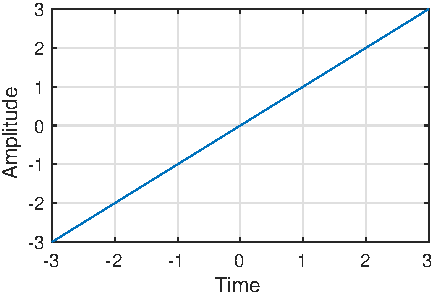
\includegraphics[width=0.5\linewidth]{images/sample-graph.pdf}
		\caption{Sample Diagram}
		\label{fig:universe}
	\end{figure}
\end{verbatim} 
which will produce the output as 
\begin{figure}[!h]
	\centering
	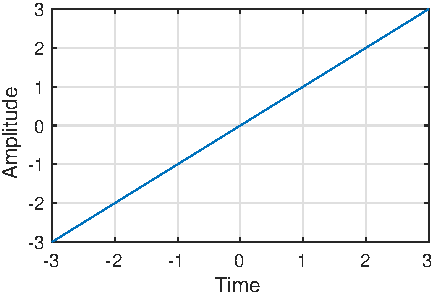
\includegraphics[width=0.5\linewidth]{images/sample-graph.pdf}
	\caption{Sample Diagram}
	\label{fig:universe1}
\end{figure}
\linebreak
More than one figures can be shown adjacent using following code
\begin{verbatim}
	\begin{figure}[h!]
		\centering
		% Left image (a)
		\begin{subfigure}[b]{0.45\linewidth}
			\centering
			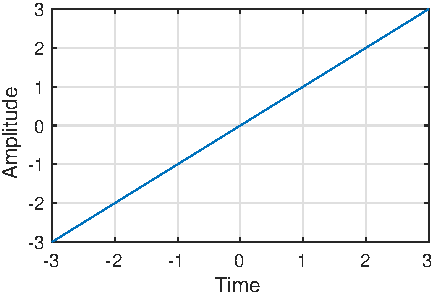
\includegraphics[width=\textwidth]{images/sample-graph.pdf} % replace with your image filename
			\caption{Example Graph}
			\label{fig:fruitsA}
		\end{subfigure}
		\hfill
		% Right image (b)
		\begin{subfigure}[b]{0.45\linewidth}
			\centering
			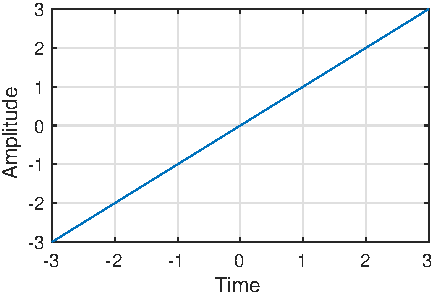
\includegraphics[width=\textwidth]{images/sample-graph.pdf} % replace with your image filename
			\caption{Example Graph}
			\label{fig:fruitsC}
		\end{subfigure}
		
		\caption{Commonly available fruits}
		\label{fig:common_fruits}
	\end{figure}
\end{verbatim}
The above code will produce the results as 
\begin{figure}[h!]
	\centering
	% Left image (a)
	\begin{subfigure}[b]{0.45\linewidth}
		\centering
		\rotatebox{45}{
		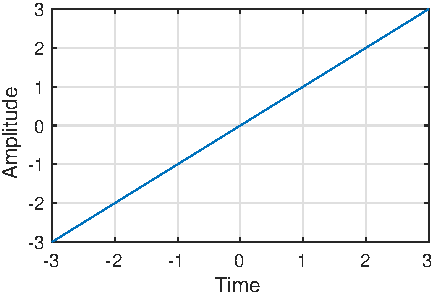
\includegraphics[width=\textwidth]{images/sample-graph.pdf} %	 replace with your image filename
		}
		
	
		\label{fig:fruitsAA}
	\end{subfigure}
	\hfill
	% Right image (b)
	\begin{subfigure}[b]{0.45\linewidth}
		\centering
		\rotatebox{-45}{
		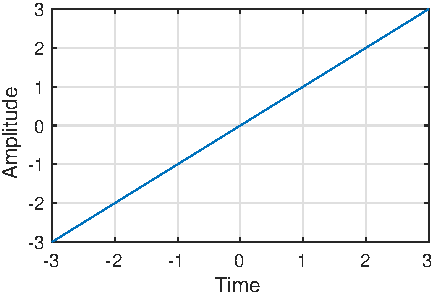
\includegraphics[width=\textwidth]{images/sample-graph.pdf} % replace with your image filename
		}
		\label{fig:fruitsCC}
	\end{subfigure}
	
	\caption{Figures with rotation}
	\label{fig:common_fruitsA}
\end{figure}

\subsection{Pseudo code / Algorithm}
The algorithm or pseudo code can be added using following code
\begin{verbatim}
	\begin{algorithm}
		\caption{An example algorithm with caption}\label{alg:cap}
		\begin{algorithmic}
			\Require $n \geq 0$
			\Ensure $y = x^n$
			\State $y \gets 1$
			\State $X \gets x$
			\State $N \gets n$
			\While{$N \neq 0$}
			\If{$N$ is even}
			\State $X \gets X \times X$
			\State $N \gets \frac{N}{2}$  \Comment{This is a comment}
			\ElsIf{$N$ is odd}
			\State $y \gets y \times X$
			\State $N \gets N - 1$
			\EndIf
			\EndWhile
		\end{algorithmic}
	\end{algorithm}
\end{verbatim}
This code will produce the following output in the report.
\begin{algorithm}
	\caption{An example algorithm with caption}\label{alg:cap}
	\begin{algorithmic}
		\Require $n \geq 0$
		\Ensure $y = x^n$
		\State $y \gets 1$
		\State $X \gets x$
		\State $N \gets n$
		\While{$N \neq 0$}
		\If{$N$ is even}
		\State $X \gets X \times X$
		\State $N \gets \frac{N}{2}$  \Comment{This is a comment}
		\ElsIf{$N$ is odd}
		\State $y \gets y \times X$
		\State $N \gets N - 1$
		\EndIf
		\EndWhile
	\end{algorithmic}
\end{algorithm}
